

\subsection{System Proposed Approach}

\subsection{System Specification}

We derive the specifications for our system based on the requirements
set by their running environments, especially those of the GUI. Since
we chose a website for this interface, the primary requirement was for
there to be a response time of under two seconds, since this is the
industry-standard benchmark \cite{akamai}, and what sites such as
Google use \cite{two-seconds}.

Response time for our website is driven by a variety of factors
typically broken down into:

\begin{itemize}
  \item The number of \emph{resources}
  \item The DNS lookup time
  \item The server response time
  \item The download time
  \item The rendering time
\end{itemize}

These times can be seen in a benchmark of an early version of our
website in figure \ref{fig-website-benchmark}.

\begin{figure}[htp]
  \centering
  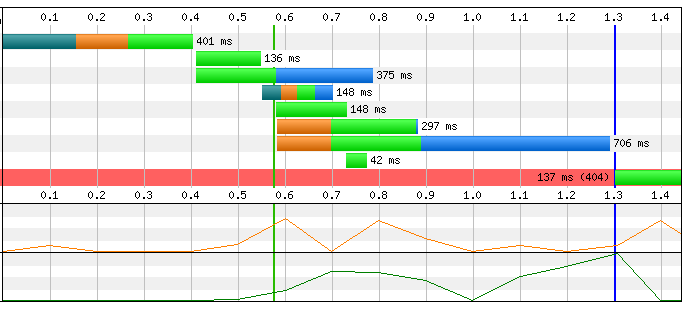
\includegraphics[height=8cm]{graphics/performance.png}
  \caption{A `Waterfall View' of the stages of a website retrieval. In
  dark green \emph{DNS Lookup}; in orange \emph{Initial Connection};
  in light green \emph{Server processing time}; in blue \emph{Download
  Time}. The green bar shows the beginning of the rendering process,
and the blue line shows the end.}
  \label{fig-website-benchmark}
\end{figure}

The main parameters under our control for this interface were the
\emph{number of resources} and \emph{download time} and the \emph{server
  response time}. Based on some experimentation, we developed the
benchmarks for the first two items shown in table \ref{specs}. The
benchmark for \emph{server response time}, as discussed above, was the
main constraint in the design of this front end, so we set the
specification for this part as high as possible while remaining
withing the overall 2 second requirement, as shown in table
\ref{specs}.

To generate the response, the server must carry out 3 tasks:

\begin{itemize}
    \item Start-up script
    \item Process user input
    \item Form response HTML
\end{itemize}

By timing a variety of CGI scripts, and comparing the results to
published benchmarks\cite{cgi-benchmark} we determined an acceptable
performance range for the start-up time. The remaining time from the
original 2 seconds was then allocated jointly to processing user input
and forming the response HTML. The requirements are set out in table
\ref{specs}.

Given the design for our overall system, [FINISH ME]


The program must handle improper input robustly and must be able to
deal with exceptions and errors gracefully. Specifically, a user of
average computer literacy should be able to understand error messages,
and, in a worst-case scenario, should be able to simply reset the
application to restore functionality.

The subsystem specifications are laid out in table \ref{specs}
\begin{table}[htp]
  \newlength\midcolumnwidth
  \midcolumnwidth=.74\textwidth plus 10\tabcolsep minus 10\tabcolsep
  \centering
  \caption{Specifications table}
  \label{specs}
  \begin{tabular}{%
    >{\raggedright}p{.11\textwidth}%
    p{\midcolumnwidth}%
    >{\raggedright\arraybackslash}p{.15\textwidth}}
  \firsthline
  \bfseries Module & \bfseries Qualitative Requirements & \bfseries
  Quantitative Performance Requirements \\ \hline
  CGI Script & Modular and correct & Memory footprint under 10 MB;
  Startup time under 50 ms \\
  \lasthline
  \end{tabular}
\end{table}
\subsection{Hardware and Software Requirements}
\subsubsection{Hardware Requirements and Design Approach}
This project did not require special hardware. Part of the
specifications of the software were that it would run on a standard
server, and it did. Furthermore, the simplicity of the website ensures
that a modest server would be able to handle the small loads.

\subsubsection{ Software Requirements and Design Approach}
The software we created was written primarily in Python, with some C
code in the back-end and Javascript for the front-end. We also chose
to use SQLite for the database work. We chose Python for the
simplicity and power of the language. By designing our system in
separate parts for the front-end and the back-end, our software
achieved the most important requirements of modularity.

Using Python enabled us to use open-source tools like
NetworkX\cite{networkx} and igraph\cite{igraph}. For the performance
critical part of our back-end, we used C to write a Python extension
that would interface with GLPK\cite{glpk}. The main reason to use C
rather than Python was the memory savings involved in the change --
each Python object cost us an incremental 16 bytes. For the SEPTA flow
solver, which had tens millions of nodes and edges the incremental
memory consumption pushed the model near the limits of a standard
computer.

The requirements we have from our software will be as follows:
\label{requirements}
\begin{description}[style=nextline]
    \item[Modularity] We should we able to switch out one
  implementation of the train model, for instance, and replace it
  seamlessly with another, more efficient implementation.
    \item[Scalability] It should be able to handle a large number of
  inputs and not break under scale. It will have to deal with tens of
  thousands of fans inhabiting the model.
    \item[User-Friendliness] We want the final output, or GUI, to be
  extremely user-friendly and it should be operational without a
  manual.
\end{description}